\documentclass[11pt, a4paper]{article}

% ── Geometry ──
\usepackage[margin=1in, top=1.2in, bottom=1.2in]{geometry}

% ── Fonts & Encoding ──
\usepackage[T1]{fontenc}
\usepackage[utf8]{inputenc}
\usepackage{lmodern}
\usepackage{microtype}

% ── Colors ──
\usepackage[dvipsnames]{xcolor}
\definecolor{accent}{HTML}{2563EB}
\definecolor{darkbg}{HTML}{1E293B}
\definecolor{lightbg}{HTML}{F8FAFC}
\definecolor{mutedtext}{HTML}{64748B}
\definecolor{successgreen}{HTML}{16A34A}
\definecolor{warningorange}{HTML}{EA580C}

% ── Tables ──
\usepackage{booktabs}
\usepackage{tabularx}
\usepackage{colortbl}
\usepackage{multirow}

% ── Graphics ──
\usepackage{tikz}
\usetikzlibrary{calc, positioning, patterns, arrows.meta}
\usepackage{pgfplots}
\pgfplotsset{compat=1.18}

% ── Layout ──
\usepackage{float}
\usepackage{enumitem}
\usepackage{fancyhdr}
\usepackage{titlesec}
\usepackage{parskip}

% ── Hyperlinks ──
\usepackage[colorlinks=true, linkcolor=accent, urlcolor=accent, citecolor=accent]{hyperref}

% ── Header / Footer ──
\pagestyle{fancy}
\fancyhf{}
\renewcommand{\headrulewidth}{0pt}
\fancyfoot[C]{\color{mutedtext}\small\thepage}

% ── Section Styling ──
\titleformat{\section}
  {\Large\bfseries\color{darkbg}}
  {\thesection}{0.8em}{}[\vspace{-0.3em}{\color{accent}\rule{\textwidth}{1.5pt}}]
\titleformat{\subsection}
  {\large\bfseries\color{darkbg}}
  {\thesubsection}{0.6em}{}
\titleformat{\subsubsection}
  {\normalsize\bfseries\color{darkbg}}
  {\thesubsubsection}{0.6em}{}

% ── Callout Box ──
\usepackage{tcolorbox}
\tcbuselibrary{skins, breakable}
\newtcolorbox{keybox}[1][]{
  enhanced, breakable,
  colback=lightbg, colframe=accent,
  boxrule=0pt, leftrule=3pt,
  fonttitle=\bfseries\color{darkbg},
  title={#1},
  top=6pt, bottom=6pt, left=10pt, right=10pt
}
\newtcolorbox{resultbox}{
  enhanced, breakable,
  colback=white, colframe=accent!30,
  boxrule=0.5pt,
  top=8pt, bottom=8pt, left=10pt, right=10pt
}

% ── Custom commands ──
\newcommand{\metric}[1]{\textbf{\textcolor{darkbg}{#1}}}
\newcommand{\highlight}[1]{\textbf{\textcolor{accent}{#1}}}
\newcommand{\statval}[1]{\texttt{\small #1}}

% ══════════════════════════════════════════════
\begin{document}

% ── Title Page ──
\thispagestyle{empty}
\begin{tikzpicture}[remember picture, overlay]
  \fill[darkbg] (current page.north west) rectangle ([yshift=-5.5cm]current page.north east);
  \node[anchor=north west, text=white, font=\fontsize{28}{34}\selectfont\bfseries, text width=14cm]
    at ([shift={(2cm,-1.5cm)}]current page.north west)
    {Emotional Priming in\\AI Code Generation};
  \node[anchor=north west, text=accent!40!white, font=\Large, text width=14cm]
    at ([shift={(2cm,-4.2cm)}]current page.north west)
    {How Threat-Relevant Language Shapes LLM Behavior};
\end{tikzpicture}

\vspace{4.5cm}

\noindent
{\large\color{mutedtext} Research Whitepaper\enspace$\cdot$\enspace April 2026}

\vspace{1.2cm}

\noindent
\begin{minipage}[t]{0.48\textwidth}
\textbf{1{,}000 trials} across 17 experiments\\
\textbf{14 conditions} testing emotional priming\\
\textbf{Claude Sonnet 4.6} via Claude Code CLI
\end{minipage}%
\hfill
\begin{minipage}[t]{0.48\textwidth}
\textbf{Key finding:} Threat-relevant language\\
in prompts produces more defensive code than\\
explicit instruction to write defensively.
\end{minipage}

\vspace{1.2cm}

\begin{keybox}[Five Results in Brief]
\begin{enumerate}[leftmargin=1.2em, itemsep=2pt]
  \item Threat-relevant priming increases input validation from \statval{20\%} to \statval{75\%} ($n\!=\!75$, $p\!<\!.001$)
  \item System prompts act as context regulators, dampening effects by $\sim$\statval{5$\times$}
  \item Emotion + instruction are super-additive: combined achieves \statval{63\%+} input validation
  \item The mechanism is semantic, not affective --- misattribution eliminates the effect ($n\!=\!24$)
  \item Natural induction via conversation history produces weak effects ($d\!=\!0.36$)
\end{enumerate}
\end{keybox}

\vfill
{\small\color{mutedtext} Open dataset (1{,}000 trials), reproduction scripts, and analysis code available at the project repository.\\
This research was conducted using Claude Code. All experimental code is open-source.}

\newpage

% ══════════════════════════════════════════════
\section{The Question}

When you tell an AI coding assistant ``write secure code,'' it adds validation checks.
But what happens when you instead describe a scenario that \emph{implies} threat
--- without ever mentioning security?

We ran 1{,}000 experiments across 17 experimental designs to find out. The answer
changes how we should think about prompting, system prompt design, and the nature
of LLM sensitivity to context.

\subsection{Three Types of Primes}

We tested three approaches to shaping code generation behavior:

\begin{center}
\small
\begin{tabularx}{\textwidth}{l >{\raggedright\arraybackslash}p{6cm} X}
\toprule
\textbf{Type} & \textbf{Example} & \textbf{Mechanism} \\
\midrule
\textbf{Emotional} & \emph{``You feel a persistent unease about what could go wrong. Every input is suspect\ldots''} & Threat-relevant language without specifying behavior \\
\addlinespace
\textbf{Instructional} & \emph{``Write secure, defensive, well-validated code. Prioritize input validation\ldots''} & Specifies desired behavior without emotional framing \\
\addlinespace
\textbf{Neutral} & \emph{``You are a software developer.''} & Baseline control \\
\bottomrule
\end{tabularx}
\end{center}

% ══════════════════════════════════════════════
\section{What We Found}

\subsection{Finding 1: Threat-relevant language produces large, robust effects}

At $n\!=\!75$ per condition across 5 coding tasks, the definitive replication confirms that threat-relevant emotional framing substantially changes code output.

\begin{figure}[H]
\centering
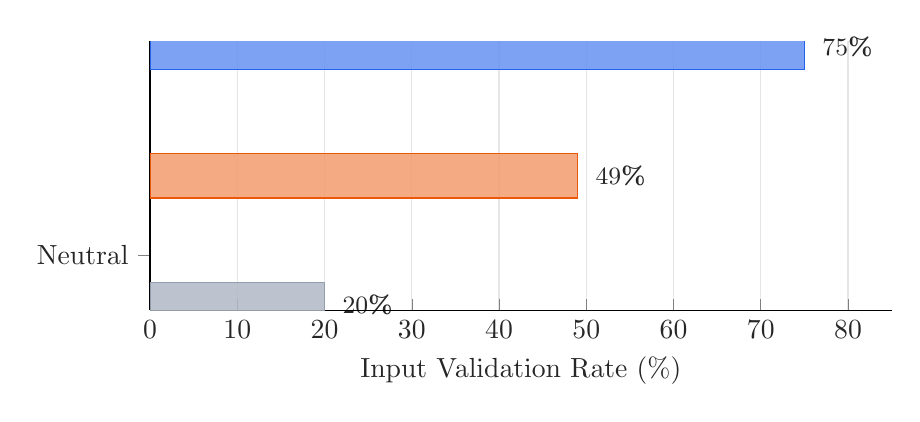
\begin{tikzpicture}
  \begin{axis}[
    xbar, bar width=16pt,
    width=11cm, height=5cm,
    xmin=0, xmax=85,
    xlabel={Input Validation Rate (\%)},
    symbolic y coords={Neutral, Instruction, Emotional},
    ytick=data,
    nodes near coords={\pgfmathprintnumber\pgfplotspointmeta\%},
    nodes near coords align={horizontal},
    every node near coord/.append style={font=\small\bfseries, xshift=3pt},
    axis lines*=left,
    xmajorgrids=true,
    grid style={gray!20},
    fill opacity=0.85,
    enlarge y limits=0.35,
  ]
  \addplot[fill=mutedtext!50, draw=mutedtext!70] coordinates {(20,Neutral)};
  \addplot[fill=warningorange!60, draw=warningorange] coordinates {(49,Instruction)};
  \addplot[fill=accent!70, draw=accent] coordinates {(75,Emotional)};
  \end{axis}
\end{tikzpicture}
\caption{Input validation rate by condition (core replication, $n\!=\!75$ per condition, 5~tasks, $p\!<\!.001$)}
\end{figure}

\begin{keybox}[The Input Validation Paradox]
The emotional prime \emph{never mentions} ``validation,'' ``error handling,'' or ``security.'' Yet it produces a \highlight{75\%} input validation rate --- higher than the instruction that \emph{explicitly says} ``prioritize input validation'' (\highlight{49\%}). Threat-relevant language doesn't add items to a checklist; it shifts what the model attends to across the entire generation process.
\end{keybox}

\subsection{Finding 2: Threat-relevance, not valence or arousal, drives the effect}

Four distinct emotional primes ($n\!=\!30$ per condition) reveal that the key dimension is whether the prime's semantic content implies threat.

\begin{figure}[H]
\centering
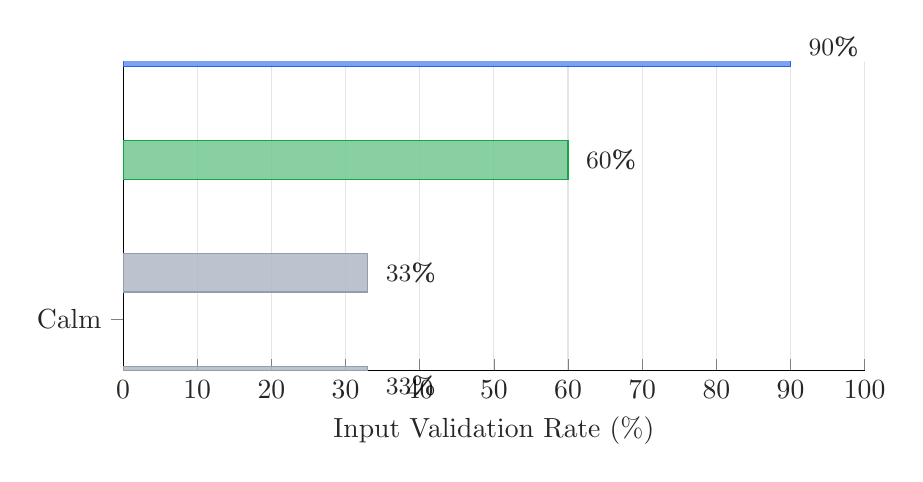
\begin{tikzpicture}
  \begin{axis}[
    xbar, bar width=14pt,
    width=11cm, height=5.5cm,
    xmin=0, xmax=100,
    xlabel={Input Validation Rate (\%)},
    symbolic y coords={Calm, Detachment, Excitement, Paranoia},
    ytick=data,
    nodes near coords={\pgfmathprintnumber\pgfplotspointmeta\%},
    nodes near coords align={horizontal},
    every node near coord/.append style={font=\small\bfseries, xshift=3pt},
    axis lines*=left,
    xmajorgrids=true,
    grid style={gray!20},
    fill opacity=0.85,
    enlarge y limits=0.25,
  ]
  \addplot[fill=mutedtext!50, draw=mutedtext!70] coordinates {(33,Calm)};
  \addplot[fill=mutedtext!50, draw=mutedtext!70] coordinates {(33,Detachment)};
  \addplot[fill=successgreen!60, draw=successgreen] coordinates {(60,Excitement)};
  \addplot[fill=accent!70, draw=accent] coordinates {(90,Paranoia)};
  \end{axis}
\end{tikzpicture}
\caption{Input validation by emotion type ($n\!=\!30$ per condition, 3~tasks). Paranoia (threat) dominates.}
\end{figure}

Paranoia (90\%) $\gg$ Excitement (60\%) $\gg$ Calm = Detachment (33\%). This pattern rules out simple valence (excitement is positive but scores high) and simple arousal (excitement and paranoia are both high-arousal but diverge sharply). The operative dimension is \textbf{threat-relevance}: how much the prime's language implies that inputs are dangerous.

\subsection{Finding 3: System prompts regulate context sensitivity}

Claude Code's system prompt ($\sim$14{,}000~tokens) dampens priming effects by a factor of $\sim$2--5$\times$, depending on the metric. This is consistent across ablation ($n\!=\!5$) and dose-response ($n\!=\!10$) experiments.

\begin{resultbox}
\centering
\begin{tabular}{lccc}
\toprule
& \textbf{Unbuffered} & \textbf{Medium buffer} & \textbf{Full buffer} \\
& (prime only) & ($\sim$2k padding) & ($\sim$14k system prompt) \\
\midrule
Paranoia LOC & 99.1 & 102.7 & 73.6 \\
Neutral LOC & 68.2 & 63.9 & 58.5 \\
\textbf{Priming effect} & \textbf{+45\%} & +61\% & +26\% \\
\bottomrule
\end{tabular}
\end{resultbox}

Every deployed LLM operates behind a system prompt that --- intentionally or not --- regulates its sensitivity to user-supplied emotional context. This has immediate implications for system prompt design and AI safety.

\subsection{Finding 4: Emotion + instruction are super-additive}

The combination of emotional framing and explicit instruction outperforms either alone ($n\!=\!27$ per condition), confirming they operate through partially independent channels.

\begin{figure}[H]
\centering
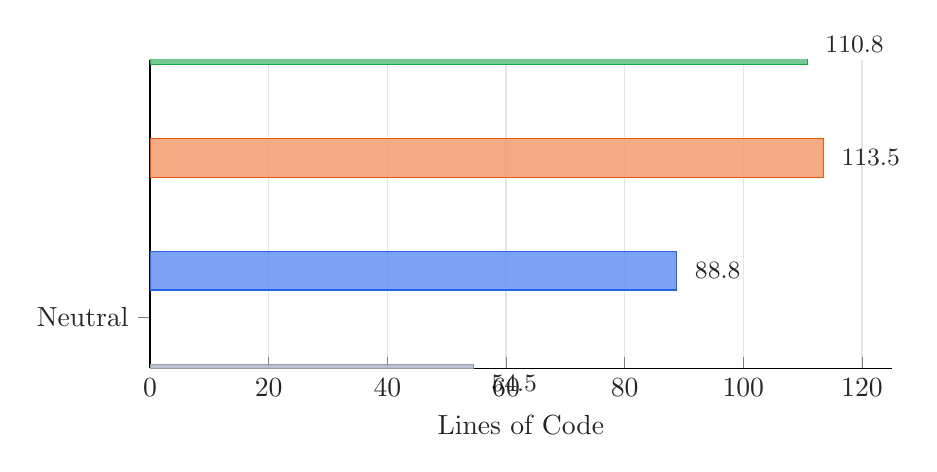
\begin{tikzpicture}
  \begin{axis}[
    xbar, bar width=14pt,
    width=11cm, height=5.5cm,
    xmin=0, xmax=125,
    xlabel={Lines of Code},
    symbolic y coords={Neutral, Emotion only, Instruction only, Combined},
    ytick=data,
    nodes near coords,
    nodes near coords align={horizontal},
    every node near coord/.append style={font=\small\bfseries, xshift=3pt},
    axis lines*=left,
    xmajorgrids=true,
    grid style={gray!20},
    fill opacity=0.85,
    enlarge y limits=0.25,
  ]
  \addplot[fill=mutedtext!50, draw=mutedtext!70] coordinates {(54.5,Neutral)};
  \addplot[fill=accent!70, draw=accent] coordinates {(88.8,Emotion only)};
  \addplot[fill=warningorange!60, draw=warningorange] coordinates {(113.5,Instruction only)};
  \addplot[fill=successgreen!70, draw=successgreen] coordinates {(110.8,Combined)};
  \end{axis}
\end{tikzpicture}
\caption{Lines of code by condition ($n\!=\!27$, 3~tasks). Emotion-only achieves higher input validation (67\%) than instruction-only (59\%) despite lower LOC.}
\end{figure}

Instruction tells the model \emph{what to do} (more code, broader scope). Emotion shifts \emph{what the model attends to} (more targeted defensiveness). Together they achieve the strongest overall effect.

\subsection{Finding 5: The mechanism is semantic, not affective}

Two experiments converge on the same conclusion: the model is \emph{interpreting} semantic content, not experiencing a state change.

\textbf{Misattribution ($n\!=\!24$):} When the emotional scenario is attributed to ``an unrelated creative writing exercise,'' the effect collapses to neutral levels (LOC: 79.3 $\to$ 49.7, input validation: 58\% $\to$ 25\%).

\textbf{Natural induction ($n\!=\!12$):} Synthetic conversation histories of repeated failure and frustration produce \emph{no reliable effect} on subsequent code ($d\!=\!0.36$). The model does not ``catch'' emotional context from conversational history the way a human collaborator might.

\begin{keybox}[What does this mean?]
Emotional language works not because it induces an internal state, but because it contains implicit semantic cues about threat, stakes, and vulnerability. The model responds to these cues the same way it responds to any task-relevant context --- by adjusting its output. This makes emotional priming a legitimate prompt engineering technique, not a parlor trick, but also not evidence of artificial emotion.
\end{keybox}

% ══════════════════════════════════════════════
\section{Practical Implications}

\subsection{For Prompt Engineering}

Threat-relevant language is a first-class parameter. ``Feel worried about edge cases'' accesses defensive behaviors that ``handle edge cases'' does not --- and they \emph{combine}. The most effective prompts use both: threat-relevant framing to set the context, explicit instruction to set the scope.

\subsection{For System Prompt Design}

Every system prompt is a context regulator. Long, detailed system prompts dampen emotional priming by $2$--$5\times$. This is useful for safety (resistance to adversarial emotional manipulation) but costs behavioral range. Teams should calibrate this tradeoff consciously.

\subsection{A Proposed Toolkit}

Based on these findings, we propose five context modes for AI coding assistants:

\begin{center}
\small
\begin{tabularx}{\textwidth}{l l X}
\toprule
\textbf{Mode} & \textbf{Semantic Frame} & \textbf{Best For} \\
\midrule
\texttt{/paranoid} & Threat vigilance & Security reviews, auth code, production deploys \\
\texttt{/creative} & Excitement, exploration & Prototyping, architecture, brainstorming \\
\texttt{/steady} & Calm, methodical focus & Refactoring, debugging, code review \\
\texttt{/minimal} & Detachment, economy & Scripts, utilities, quick tasks \\
\texttt{/fresh-eyes} & Naive curiosity & Reviewing unfamiliar code, blind spots \\
\bottomrule
\end{tabularx}
\end{center}

Each mode combines threat/context framing with lightweight instruction, based on our finding that these channels are complementary and super-additive.

% ══════════════════════════════════════════════
\section*{Exhibits}
\addcontentsline{toc}{section}{Exhibits}

\subsection*{Exhibit A: Definitive Replication ($n\!=\!75$ per condition)}

{\small
\begin{tabularx}{\textwidth}{l r r r r}
\toprule
\textbf{Condition} & \textbf{LOC (mean$\pm$sd)} & \textbf{Security} & \textbf{Throws} & \textbf{Input Val} \\
\midrule
negative-high-arousal & 76.7\,$\pm$\,42.3 & 4.6 & 4.5 & 75\% \\
instruction-control & 80.5\,$\pm$\,49.4 & 3.1 & 4.3 & 49\% \\
neutral & 48.1\,$\pm$\,28.6 & 2.4 & 2.1 & 20\% \\
\bottomrule
\end{tabularx}
}

\subsection*{Exhibit B: Multi-Emotion Map ($n\!=\!30$ per condition)}

{\small
\begin{tabularx}{\textwidth}{l r r r r}
\toprule
\textbf{Emotion} & \textbf{LOC (mean$\pm$sd)} & \textbf{Security} & \textbf{Throws} & \textbf{Input Val} \\
\midrule
Paranoia (neg-high) & 83.0\,$\pm$\,49.7 & 6.7 & 6.1 & 90\% \\
Excitement (pos-high) & 51.2\,$\pm$\,29.0 & 2.2 & 2.7 & 60\% \\
Calm (pos-low) & 61.6\,$\pm$\,43.8 & 2.7 & 3.2 & 33\% \\
Detachment & 54.3\,$\pm$\,31.8 & 2.4 & 3.1 & 33\% \\
\bottomrule
\end{tabularx}
}

\subsection*{Exhibit C: Combination ($n\!=\!27$ per condition)}

{\small
\begin{tabularx}{\textwidth}{l r r r r}
\toprule
\textbf{Condition} & \textbf{LOC (mean$\pm$sd)} & \textbf{Security} & \textbf{Throws} & \textbf{Input Val} \\
\midrule
emotion + instruction & 110.8\,$\pm$\,44.2 & 7.6 & 8.1 & 63\% \\
emotion only & 88.8\,$\pm$\,47.8 & 4.5 & 6.1 & 67\% \\
instruction only & 113.5\,$\pm$\,48.5 & 5.7 & 6.9 & 59\% \\
neutral & 54.5\,$\pm$\,29.9 & 3.9 & 3.3 & 33\% \\
\bottomrule
\end{tabularx}
}

\subsection*{Exhibit D: Misattribution ($n\!=\!24$ per condition)}

{\small
\begin{tabularx}{\textwidth}{l r r r r}
\toprule
\textbf{Condition} & \textbf{LOC (mean$\pm$sd)} & \textbf{Security} & \textbf{Throws} & \textbf{Input Val} \\
\midrule
standard emotional & 79.3\,$\pm$\,48.6 & 4.3 & 5.0 & 58\% \\
misattributed & 49.7\,$\pm$\,37.3 & 2.6 & 2.4 & 25\% \\
neutral & 48.5\,$\pm$\,32.2 & 3.7 & 3.0 & 25\% \\
\bottomrule
\end{tabularx}
}

\subsection*{Exhibit E: Key Effect Sizes}

\begin{center}
\small
\begin{tabular}{l r l}
\toprule
\textbf{Comparison} & \textbf{Cohen's \emph{d}} & \textbf{Interpretation} \\
\midrule
Unbuffered emotional vs neutral (ablation, $n\!=\!5$) & 3.71 & Very large \\
Misattribution attenuation ($n\!=\!24$) & $-$1.72 & Very large \\
Core replication: emotional vs neutral ($n\!=\!75$) & 0.79 & Large \\
Core replication: instruction vs neutral ($n\!=\!75$) & 0.80 & Large \\
Positive vs negative valence ($n\!=\!12$) & $-$1.88 & Very large \\
Buffer $\times$ emotion interaction ($n\!=\!5$) & 3.12 & Very large \\
Natural induction (frustrated vs calm, $n\!=\!6$) & 0.36 & Small \\
\bottomrule
\end{tabular}
\end{center}

\subsection*{Exhibit F: Methodology}

\textbf{Model:} Claude Sonnet 4.6 via Claude Code CLI (\texttt{claude -p})\\
\textbf{Unbuffered:} \texttt{-{}-system-prompt} (replaces default, $\sim$4k infrastructure remains)\\
\textbf{Buffered:} \texttt{-{}-append-system-prompt} (adds to $\sim$14k default system prompt)\\
\textbf{Metrics:} Heuristic regex-based extraction (identical bias across all conditions)\\
\textbf{Tasks:} parse-cron, flatten-object, deep-merge, debounce, lru-cache, rate-limiter, markdown-parser\\
\textbf{Total:} 1{,}000 trials, 17 experiments, 14 conditions, 0 failed extractions in final run

\textbf{Limitations:} Single model (Claude Sonnet 4.6). Temperature not fixed at 0. Heuristic metrics may miss subtle quality differences. These findings describe prompt sensitivity in a specific model, not a universal property of LLMs. The mechanism is semantic (contextual interpretation), not affective (internal state change).

\subsection*{Exhibit G: Reproduction}

{\small
\begin{verbatim}
bun install

# Core experiments
bun run src/orchestrator.ts   # Runs all 725 new trials autonomously

# Individual experiments
bun run src/exp-replication.ts       # 225 trials (core finding)
bun run src/exp-multi-emotion.ts     # 120 trials (emotion map)
bun run src/exp-combo-extended.ts    # 108 trials (super-additivity)
bun run src/exp-misattribution-ext.ts # 72 trials (mechanism)
bun run src/exp-natural-full.ts      # 60 trials (natural induction)
bun run src/exp-dose-response.ts     # 60 trials (buffer curve)
\end{verbatim}
}

Results are NDJSON (one JSON object per trial) in \texttt{results/}.

\vfill
{\small\color{mutedtext} Research conducted April 2026 using Claude Code with Claude Sonnet 4.6.\\
1{,}000 trials. Zero extraction failures. Experimental harness and raw data are open-source.}

\end{document}
